% Complex Tori and Elliptic Curves --- COMPANION GALLERY (A0 portrait).
% Page 1 (poster.tex) carries the argument and is full; this second sheet collects six
% further TikZ visualizations of the same object.  Shares figuremacros/palette and the
% Sage coordinates.  Build:  pdflatex poster_gallery.tex  (twice).
\documentclass[25pt, a0paper, portrait, margin=14mm, innermargin=15mm,
               blockverticalspace=14mm, colspace=18mm, subcolspace=8mm]{tikzposter}

\usepackage{amsmath,amssymb,mathtools}

% figuremacros.tex --- figure infrastructure harvested from book/preamble.tex
% (TikZ libraries, the form* colour palette, the three \drawprecise macros,
%  and the diagram tikzset). Do not edit; mirror of the book's definitions.

\usetikzlibrary{arrows.meta,calc,positioning,decorations.markings,decorations.pathmorphing,
  patterns,shadings,shapes.geometric,fadings,backgrounds,intersections,bending}

\definecolor{formteal}{HTML}{1f4e79}
\definecolor{formgold}{HTML}{b88a14}
\definecolor{formrust}{HTML}{a8431d}
\definecolor{formplum}{HTML}{6b2e6e}
\definecolor{formsage}{HTML}{467b3a}
\definecolor{formslate}{HTML}{3a5168}
\definecolor{formivory}{HTML}{f6efe0}

\newcommand{\drawprecisetorus}{%
  % (1) Fill the visible torus body with light teal.
  \fill[formteal!13, line join=round]
    plot[smooth cycle] coordinates {\torusOuter};
  % (2) Cut out the donut hole using the inner silhouette curve.
  \fill[white, line join=round]
    plot[smooth cycle] coordinates {\torusInner};
  % (3) Visible meridian arcs (eight small circles spaced 45 deg apart).
  % Back meridians (v in [0, pi]) form one visible arc each;
  % front meridians (v in (pi, 2 pi)) wrap across u = 0 and are split
  % into two visible chunks (VA and VB) by the sampling boundary.
  \draw[draw=formteal!60!black, line width=0.42pt, line join=round, opacity=0.9]
    plot[smooth] coordinates {\torusMerZeroVA};
  \draw[draw=formteal!60!black, line width=0.42pt, line join=round, opacity=0.9]
    plot[smooth] coordinates {\torusMerOneVA};
  \draw[draw=formteal!60!black, line width=0.42pt, line join=round, opacity=0.9]
    plot[smooth] coordinates {\torusMerTwoVA};
  \draw[draw=formteal!60!black, line width=0.42pt, line join=round, opacity=0.9]
    plot[smooth] coordinates {\torusMerThreeVA};
  \draw[draw=formteal!60!black, line width=0.42pt, line join=round, opacity=0.9]
    plot[smooth] coordinates {\torusMerFourVA};
  \draw[draw=formteal!60!black, line width=0.42pt, line join=round, opacity=0.9]
    plot[smooth] coordinates {\torusMerFiveVA};
  \draw[draw=formteal!60!black, line width=0.42pt, line join=round, opacity=0.9]
    plot[smooth] coordinates {\torusMerFiveVB};
  \draw[draw=formteal!60!black, line width=0.42pt, line join=round, opacity=0.9]
    plot[smooth] coordinates {\torusMerSixVA};
  \draw[draw=formteal!60!black, line width=0.42pt, line join=round, opacity=0.9]
    plot[smooth] coordinates {\torusMerSixVB};
  \draw[draw=formteal!60!black, line width=0.42pt, line join=round, opacity=0.9]
    plot[smooth] coordinates {\torusMerSevenVA};
  \draw[draw=formteal!60!black, line width=0.42pt, line join=round, opacity=0.9]
    plot[smooth] coordinates {\torusMerSevenVB};
  % (4) Visible longitude arcs (the four canonical latitude circles).
  % Outer (u=0) is visible only on the front half (v in (pi, 2 pi)),
  % inner (u=pi) only on the back half (v in (0, pi)); the top crest
  % (u=pi/2) is visible everywhere; the bottom (u=3pi/2) is fully hidden.
  \draw[draw=formteal!60!black, line width=0.5pt, line join=round, opacity=0.95]
    plot[smooth] coordinates {\torusLonTopVA};
  \draw[draw=formteal!60!black, line width=0.42pt, line join=round, opacity=0.8]
    plot[smooth] coordinates {\torusLonOuterVA};
  \draw[draw=formteal!60!black, line width=0.42pt, line join=round, opacity=0.8]
    plot[smooth] coordinates {\torusLonInnerVA};
  % (5) Crisp silhouette outlines drawn last so they sit on top.
  \draw[draw=formteal!65!black, line width=0.95pt, line join=round]
    plot[smooth cycle] coordinates {\torusOuter};
  \draw[draw=formteal!65!black, line width=0.8pt, line join=round]
    plot[smooth cycle] coordinates {\torusInner};
}

\newcommand{\drawprecisesphere}{%
  % Color tone matches the torus (formteal) for visual unity across figures.
  % (1) Flat-filled body of the sphere (same filling style as the torus)
  \fill[formteal!13, line join=round]
    plot[smooth cycle] coordinates {\sphereOutline};
  % (2) Visible latitude arcs
  \draw[draw=formteal!60!black, line width=0.45pt, line join=round, opacity=0.9]
    plot[smooth] coordinates {\sphereLatEquatorVA};
  \draw[draw=formteal!60!black, line width=0.4pt, line join=round, opacity=0.85]
    plot[smooth] coordinates {\sphereLatNorthVA};
  \draw[draw=formteal!60!black, line width=0.4pt, line join=round, opacity=0.85]
    plot[smooth] coordinates {\sphereLatNorthVB};
  \draw[draw=formteal!60!black, line width=0.4pt, line join=round, opacity=0.85]
    plot[smooth] coordinates {\sphereLatTropicVA};
  \draw[draw=formteal!60!black, line width=0.4pt, line join=round, opacity=0.85]
    plot[smooth] coordinates {\sphereLatTropicVB};
  \draw[draw=formteal!60!black, line width=0.4pt, line join=round, opacity=0.85]
    plot[smooth] coordinates {\sphereLatSouthVA};
  % (3) Visible meridian arcs (eight meridians at v = k pi/4)
  \draw[draw=formteal!60!black, line width=0.42pt, line join=round, opacity=0.9]
    plot[smooth] coordinates {\sphereMerZeroVA};
  \draw[draw=formteal!60!black, line width=0.42pt, line join=round, opacity=0.9]
    plot[smooth] coordinates {\sphereMerOneVA};
  \draw[draw=formteal!60!black, line width=0.42pt, line join=round, opacity=0.9]
    plot[smooth] coordinates {\sphereMerTwoVA};
  \draw[draw=formteal!60!black, line width=0.42pt, line join=round, opacity=0.9]
    plot[smooth] coordinates {\sphereMerThreeVA};
  \draw[draw=formteal!60!black, line width=0.42pt, line join=round, opacity=0.9]
    plot[smooth] coordinates {\sphereMerFourVA};
  \draw[draw=formteal!60!black, line width=0.42pt, line join=round, opacity=0.9]
    plot[smooth] coordinates {\sphereMerFiveVA};
  \draw[draw=formteal!60!black, line width=0.42pt, line join=round, opacity=0.9]
    plot[smooth] coordinates {\sphereMerSixVA};
  \draw[draw=formteal!60!black, line width=0.42pt, line join=round, opacity=0.9]
    plot[smooth] coordinates {\sphereMerSevenVA};
  % (4) Hidden back arcs as dashed light strokes
  \draw[draw=formteal!50!black, dashed, line width=0.3pt, line join=round, opacity=0.55]
    plot[smooth] coordinates {\sphereLatEquatorHA};
  % (5) Crisp silhouette outline on top
  \draw[draw=formteal!65!black, line width=0.95pt, line join=round]
    plot[smooth cycle] coordinates {\sphereOutline};
}

\newcommand{\drawprecisecurve}{%
  % Oval (compact component, x in [-1,0]): draw as closed smooth cycle.
  \draw[draw=formteal!60!black, line width=0.88pt, line join=round]
    plot[smooth cycle, tension=0.85] coordinates {\curveOvalFull};
  % Branch (unbounded component, x >= 1): upper and lower arcs.
  \draw[draw=formteal!60!black, line width=0.88pt, line join=round]
    plot[smooth, tension=0.9] coordinates {\curveBranchUpper};
  \draw[draw=formteal!60!black, line width=0.88pt, line join=round]
    plot[smooth, tension=0.9] coordinates {\curveBranchLower};
  % Branch points (Weierstrass roots e1=-1, e2=0, e3=1)
  \fill[formteal!70!black] (-1,0) circle (1.8pt);
  \fill[formteal!70!black] ( 0,0) circle (1.8pt);
  \fill[formteal!70!black] ( 1,0) circle (1.8pt);
}

\tikzset{
  arrow/.style={-{Latex[length=2mm]}, thick},
  point/.style={circle, fill=black, inner sep=1.5pt},
  labelnode/.style={font=\small, align=center},
  note/.style={draw=black!55, rounded corners=2pt, align=center, inner sep=5pt, fill=black!3},
  visualnode/.style={draw=black!60, rounded corners=2pt, align=center, inner sep=6pt, fill=black!2}
}


\newcommand{\C}{\mathbb{C}}
\newcommand{\R}{\mathbb{R}}
\newcommand{\Z}{\mathbb{Z}}
\newcommand{\Q}{\mathbb{Q}}
\newcommand{\F}{\mathbb{F}}
\newcommand{\CP}{\mathbb{CP}}
\newcommand{\HH}{\mathbb{H}}

\newcommand{\sagedir}{../sagemath}
\input{\sagedir/coords.tex}

\definecolorstyle{book}{}{%
  \colorlet{backgroundcolor}{formivory!55}%
  \colorlet{framecolor}{formteal!70!black}%
}{%
  \colorlet{titlefgcolor}{formivory}%
  \colorlet{titlebgcolor}{formteal!88!black}%
}{%
  \colorlet{blocktitlebgcolor}{formteal}%
  \colorlet{blocktitlefgcolor}{white}%
  \colorlet{blockbodybgcolor}{white}%
  \colorlet{blockbodyfgcolor}{black}%
}{%
  \colorlet{innerblocktitlebgcolor}{formgold}%
  \colorlet{innerblocktitlefgcolor}{black}%
  \colorlet{innerblockbodybgcolor}{formgold!18}%
  \colorlet{innerblockbodyfgcolor}{black}%
}{%
  \colorlet{notefgcolor}{black}%
  \colorlet{notebgcolor}{formgold!22}%
  \colorlet{notefrcolor}{formgold!80!black}%
}
\usetheme{Default}
\usecolorstyle{book}

\newcommand{\figH}[2]{\par\smallskip{\centering\resizebox{!}{#1}{#2}\par}\smallskip}
\newcommand{\figcap}[1]{{\centering\small\itshape #1\par}\smallskip}

\title{Complex Tori and Elliptic Curves}
\author{Companion Gallery --- six further pictures of the same object}
\institute{Read alongside the main poster: the real and finite faces of $E$, the torsion and moduli structure, and the degenerations}
\makeatletter
\settitle{%
  \centering\color{titlefgcolor}%
  {\fontsize{56}{64}\selectfont\bfseries \@title}\\[0.30em]
  {\fontsize{28}{34}\selectfont \@author}\\[0.18em]
  {\fontsize{22}{27}\selectfont\itshape \@institute}%
}
\makeatother

\begin{document}
\maketitle[width=\textwidth]

\block{\large Gallery --- More Pictures of the Same Story}{%
\normalsize
The main poster carries the argument that the chord--tangent law on a cubic \emph{is}
addition on the torus $\C/\Lambda$. This companion sheet enriches it with six further
pictures of the \emph{same} object: the real and finite-field faces of $E$, the second
Weierstrass function $\wp'$, the torsion and moduli structure, and the degenerations that
force the discriminant $\Delta\neq0$.}

\begin{columns}

\column{0.5}

\block{\large The real picture: two components}{%
\figH{380pt}{% Real points of E: y^2 = 4x^3 - 4x.  Two components -- a compact oval over [e1,e2] and an
% unbounded branch over [e3, infty) meeting at O at infinity.  The three roots together
% with O form the 2-torsion E[2] = {O, e1, e2, e3} = (Z/2)^2.
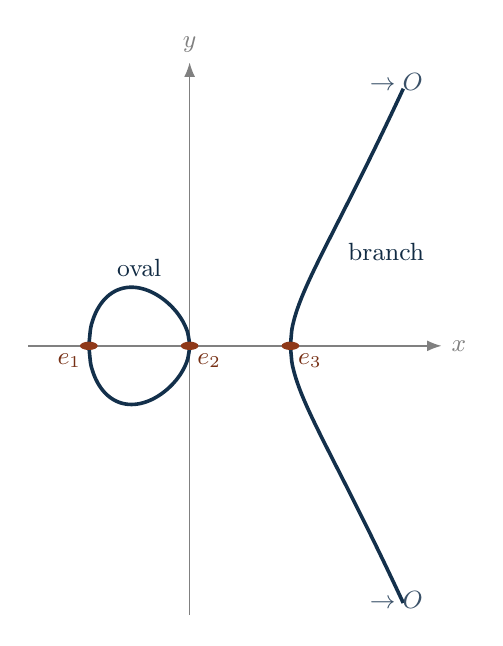
\begin{tikzpicture}[>=Latex, xscale=1.28, yscale=0.6]
  \draw[->, black!50, line width=0.5pt] (-1.6,0)--(2.5,0) node[right, font=\small] {$x$};
  \draw[->, black!50, line width=0.5pt] (0,-5.7)--(0,6.0) node[above, font=\small] {$y$};
  \draw[formteal!62!black, line width=1.3pt, smooth, samples=60, domain=-1:0]
    plot (\x,{ 2*sqrt(max(\x*\x*\x-\x,0))});
  \draw[formteal!62!black, line width=1.3pt, smooth, samples=60, domain=-1:0]
    plot (\x,{-2*sqrt(max(\x*\x*\x-\x,0))});
  \draw[formteal!62!black, line width=1.3pt, smooth, samples=80, domain=1:2.12]
    plot (\x,{ 2*sqrt(max(\x*\x*\x-\x,0))});
  \draw[formteal!62!black, line width=1.3pt, smooth, samples=80, domain=1:2.12]
    plot (\x,{-2*sqrt(max(\x*\x*\x-\x,0))});
  \foreach \r in {-1,0,1}{\fill[formrust!85!black] (\r,0) circle (2.5pt);}
  \node[below left=-1pt, font=\small, formrust!70!black] at (-1,0) {$e_1$};
  \node[below right=-1pt, font=\small, formrust!70!black] at (0,0) {$e_2$};
  \node[below right=-1pt, font=\small, formrust!70!black] at (1,0) {$e_3$};
  \node[formteal!55!black, font=\small] at (-0.5,1.65) {oval};
  \node[formteal!55!black, font=\small] at (1.95,2.0) {branch};
  \node[formslate, font=\small, anchor=south] at (2.05,5.2) {$\to O$};
  \node[formslate, font=\small, anchor=north] at (2.05,-5.0) {$\to O$};
\end{tikzpicture}
}
\figcap{Over $\R$, $E:\,y^2=4x^3-4x$ has a compact \emph{oval} over $[e_1,e_2]$ and an
\emph{unbounded branch} over $[e_3,\infty)$, both ends running to $O$ at infinity. The
three roots together with $O$ are the $2$-torsion $E[2]=\{O,e_1,e_2,e_3\}\cong(\Z/2\Z)^2$.}}

\block{\large Torsion: $E[n]\cong(\Z/n\Z)^2$}{%
\figH{330pt}{% The n-torsion E[n] = (1/n)Lambda / Lambda is a regular n x n grid inside one tile,
% so E[n] = (Z/nZ)^2.  Shown for n=3: the 9 three-torsion points (the flexes of E).
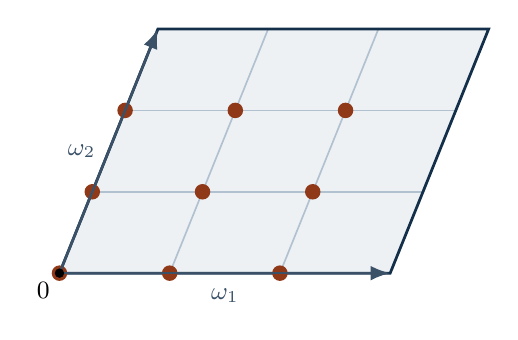
\begin{tikzpicture}[>=Latex]
  \def\ax{4.2}\def\bx{1.25}\def\by{3.1}
  \fill[formteal!8] (0,0)--(\ax,0)--(\ax+\bx,\by)--(\bx,\by)--cycle;
  % sub-grid at thirds
  \foreach \k in {1,2}{
    \draw[formteal!35, line width=0.6pt]
      ({\k/3*\ax},0)--({\k/3*\ax+\bx},\by);
    \draw[formteal!35, line width=0.6pt]
      ({\k/3*\bx},{\k/3*\by})--({\ax+\k/3*\bx},{\k/3*\by});}
  \draw[formteal!60!black, line width=1pt] (0,0)--(\ax,0)--(\ax+\bx,\by)--(\bx,\by)--cycle;
  % the 9 three-torsion points
  \foreach \a in {0,1,2}{\foreach \b in {0,1,2}{
    \fill[formrust!85!black] ({\a/3*\ax+\b/3*\bx},{\b/3*\by}) circle (2.8pt);}}
  \draw[->, formslate, line width=0.9pt] (0,0)--(\ax,0)
    node[midway, below=2pt, font=\small] {$\omega_1$};
  \draw[->, formslate, line width=0.9pt] (0,0)--(\bx,\by)
    node[midway, left=1pt, font=\small] {$\omega_2$};
  \fill[black] (0,0) circle (1.7pt) node[below left, font=\small] {$0$};
\end{tikzpicture}
}
\figcap{The $n$-torsion is $\tfrac1n\Lambda/\Lambda$ --- a regular $n\times n$ grid inside
one tile, so $E[n]\cong(\Z/n\Z)^2$. Shown for $n=3$: the nine three-torsion points,
exactly the flexes of $E$.}}

\block{\large Over a finite field: $E(\F_7)$}{%
\figH{360pt}{% The same rational group law works over a finite field.  E(F_7): y^2 = 4x^3 - 4x over
% F_7 has the 7 affine points below plus O, eight in all; the points with y=0 (x=0,1,6)
% are the 2-torsion.  (Point set verified with python.)
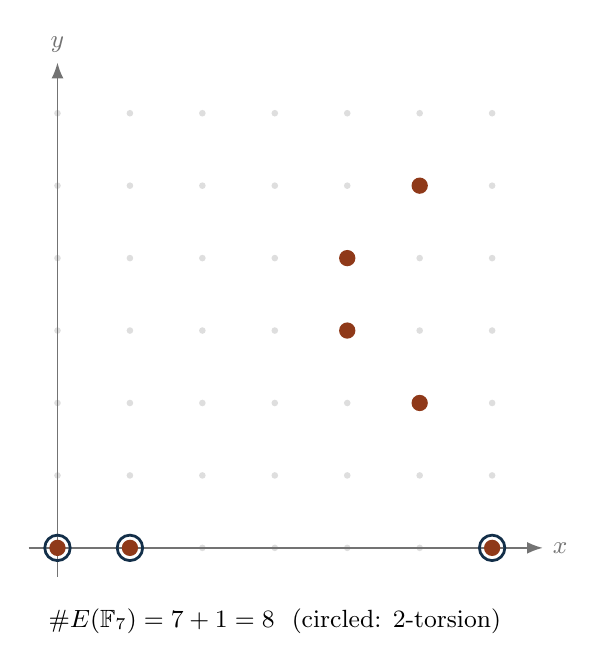
\begin{tikzpicture}[>=Latex, scale=0.92]
  \foreach \x in {0,...,6}{\foreach \y in {0,...,6}{\fill[black!13] (\x,\y) circle (1.3pt);}}
  \draw[->, black!55, line width=0.6pt] (-0.4,0)--(6.7,0) node[right, font=\small] {$x$};
  \draw[->, black!55, line width=0.6pt] (0,-0.4)--(0,6.7) node[above, font=\small] {$y$};
  \foreach \x/\y in {0/0, 1/0, 6/0, 4/3, 4/4, 5/2, 5/5}{
    \fill[formrust!85!black] (\x,\y) circle (3.2pt);}
  \foreach \x in {0,1,6}{\draw[formteal!60!black, line width=1pt] (\x,0) circle (5pt);}
  \node[font=\small, anchor=north] at (3,-0.7) {$\#E(\F_7)=7+1=8$ \ (circled: $2$-torsion)};
\end{tikzpicture}
}
\figcap{Because the addition law is \emph{rational}, it works mod $p$. Solving
$y^2=4x^3-4x$ over $\F_7$ gives seven affine points; with $O$, $\#E(\F_7)=8$. The full
$2$-torsion (circled) makes $E(\F_7)\cong\Z/2\oplus\Z/4$.}}

\column{0.5}

\block{\large The other function: $\wp'$}{%
\figH{325pt}{% The companion graph: wp' on the real axis.  Odd, with a triple pole at every lattice
% point, vanishing at the half-periods (where wp has its extrema).  The pair (wp, wp')
% is exactly the (x, y) of the embedding.  (Truncated lattice sum, clipped to the box.)
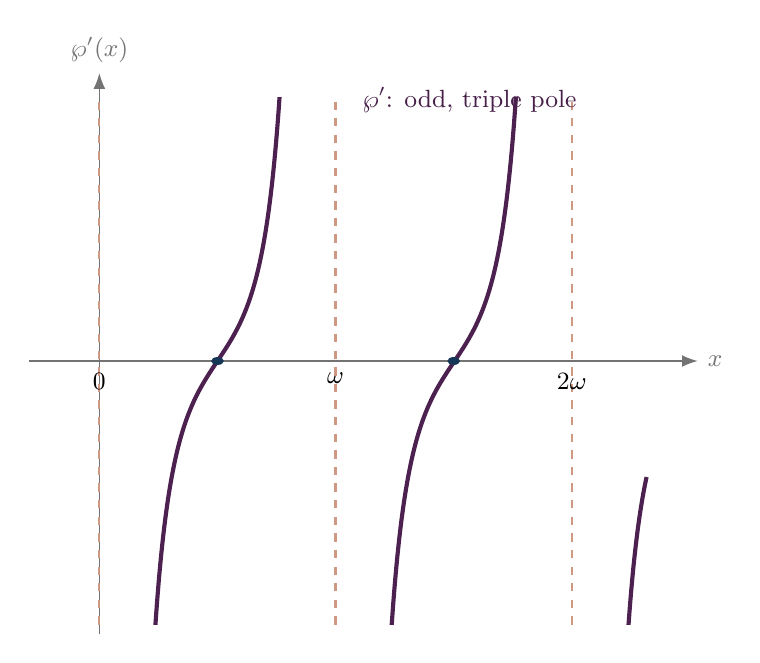
\begin{tikzpicture}[>=Latex, yscale=0.62]
  \draw[->, black!55, line width=0.6pt] (-0.9,0)--(7.6,0) node[right, font=\small] {$x$};
  \draw[->, black!55, line width=0.6pt] (0,-5.6)--(0,5.9) node[above, font=\small] {$\wp'(x)$};
  \foreach \p in {0,3,6}{\draw[formrust!55, dashed, line width=0.8pt] (\p,-5.4)--(\p,5.4);}
  \begin{scope}
    \clip (-0.9,-5.4) rectangle (7.6,5.4);
    \foreach \lo/\hi in {0.6/2.4, 3.6/5.4, 6.6/6.95}{
      \draw[formplum!72!black, line width=1.5pt, smooth, samples=70, domain=\lo:\hi]
        plot (\x,{-2*( 1/(\x*\x*\x) + 1/((\x-3)*(\x-3)*(\x-3))
                     + 1/((\x+3)*(\x+3)*(\x+3)) + 1/((\x-6)*(\x-6)*(\x-6)) )});}
  \end{scope}
  \foreach \h in {1.5,4.5}{\fill[formteal!70!black] (\h,0) circle (2.3pt);}
  \node[font=\small, below] at (0,-0.05) {$0$};
  \node[font=\small, below] at (3,-0.05) {$\omega$};
  \node[font=\small, below] at (6,-0.05) {$2\omega$};
  \node[formplum!65!black, font=\small, anchor=south] at (4.7,4.9) {$\wp'$: odd, triple pole};
\end{tikzpicture}
}
\figcap{Beside $\wp$ lives its derivative $\wp'$: odd, with a \emph{triple} pole at every
lattice point, vanishing at the half-periods (where $\wp$ has its extrema). The pair
$(\wp,\wp')$ is precisely the $(x,y)$ of the embedding $\Phi=[\wp:\wp':1]$.}}

\block{\large Moduli: shape sets the $j$-invariant}{%
\figH{260pt}{% Different lattice shapes give non-isomorphic tori, told apart by the j-invariant:
% the square lattice (tau=i, j=1728) and the hexagonal lattice (tau=rho, j=0) are the
% two extra-symmetric ones; a generic tau gives a generic j.
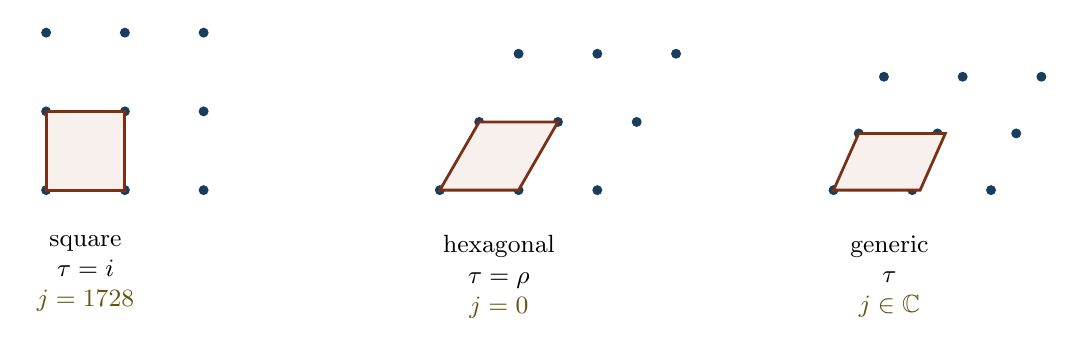
\begin{tikzpicture}[>=Latex]
  % square, tau = i
  \begin{scope}[xshift=0cm]
    \foreach \i in {0,1,2}{\foreach \j in {0,1,2}{\fill[formteal!78!black] (\i,\j) circle (1.8pt);}}
    \draw[formrust!72!black, line width=1pt, fill=formrust!8] (0,0)--(1,0)--(1,1)--(0,1)--cycle;
    \node[align=center, font=\small, anchor=north] at (0.5,-0.45)
      {square\\$\tau=i$\\{\color{formgold!58!black}$j=1728$}};
  \end{scope}
  % hexagonal, tau = rho
  \begin{scope}[xshift=5.0cm]
    \foreach \i in {0,1,2}{\foreach \j in {0,1,2}{\fill[formteal!78!black] ({\i+0.5*\j},{0.866*\j}) circle (1.8pt);}}
    \draw[formrust!72!black, line width=1pt, fill=formrust!8] (0,0)--(1,0)--(1.5,0.866)--(0.5,0.866)--cycle;
    \node[align=center, font=\small, anchor=north] at (0.75,-0.45)
      {hexagonal\\$\tau=\rho$\\{\color{formgold!58!black}$j=0$}};
  \end{scope}
  % generic
  \begin{scope}[xshift=10.0cm]
    \foreach \i in {0,1,2}{\foreach \j in {0,1,2}{\fill[formteal!78!black] ({\i+0.32*\j},{0.72*\j}) circle (1.8pt);}}
    \draw[formrust!72!black, line width=1pt, fill=formrust!8] (0,0)--(1.1,0)--(1.42,0.72)--(0.32,0.72)--cycle;
    \node[align=center, font=\small, anchor=north] at (0.71,-0.45)
      {generic\\$\tau$\\{\color{formgold!58!black}$j\in\C$}};
  \end{scope}
\end{tikzpicture}
}
\figcap{Homothetic lattices give the same torus; the shape $\tau\in\HH$, taken modulo
$\mathrm{SL}_2(\Z)$, is recorded by the $j$-invariant. The square ($\tau=i$, $j=1728$) and
hexagonal ($\tau=\rho$, $j=0$) lattices are the two extra-symmetric ones.}}

\block{\large Why $\Delta\neq0$: node and cusp}{%
\figH{310pt}{% Why we insist on Delta != 0.  As the discriminant degenerates, the smooth cubic (a
% torus) collapses: two roots colliding give a node (group C^*), a triple root gives a
% cusp (group C).  Only the smooth case is an elliptic curve.
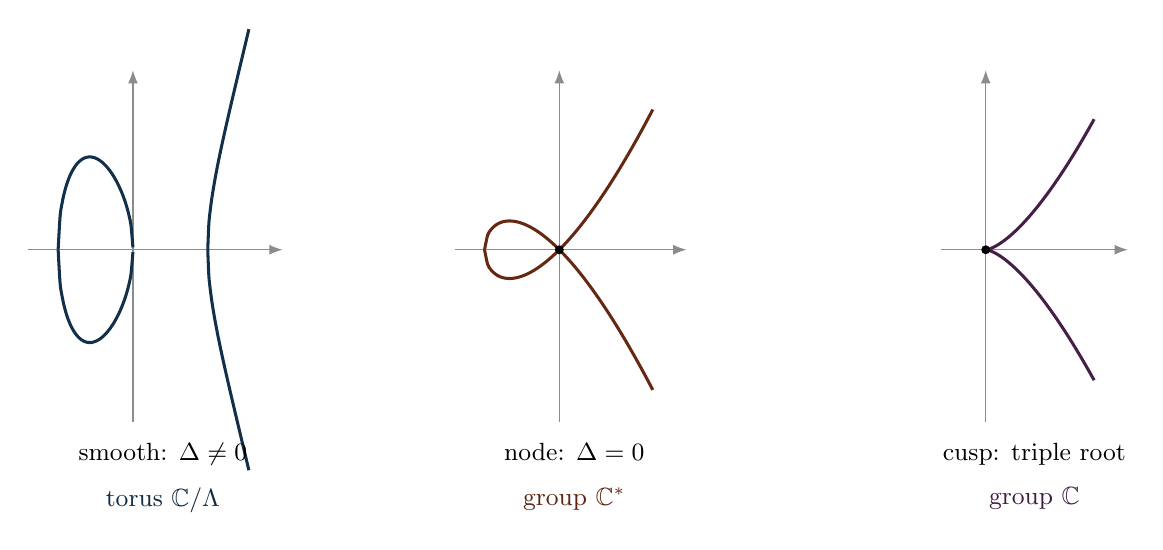
\begin{tikzpicture}[>=Latex, scale=0.95]
  % smooth: y^2 = x^3 - x
  \begin{scope}[xshift=0cm]
    \draw[->, black!45, line width=0.4pt] (-1.4,0)--(2.0,0);
    \draw[->, black!45, line width=0.4pt] (0,-2.3)--(0,2.4);
    \foreach \s in {1,-1}{
      \draw[formteal!62!black, line width=1.1pt, smooth, samples=40, domain=-1:0]
        plot (\x,{\s*2*sqrt(max(\x*\x*\x-\x,0))});
      \draw[formteal!62!black, line width=1.1pt, smooth, samples=40, domain=1:1.55]
        plot (\x,{\s*2*sqrt(max(\x*\x*\x-\x,0))});}
    \node[font=\small, anchor=north] at (0.4,-2.45) {smooth: $\Delta\ne0$};
    \node[font=\small, formteal!55!black, anchor=north] at (0.4,-3.05) {torus $\C/\Lambda$};
  \end{scope}
  % node: y^2 = x^2 (x+1)
  \begin{scope}[xshift=5.7cm]
    \draw[->, black!45, line width=0.4pt] (-1.4,0)--(1.7,0);
    \draw[->, black!45, line width=0.4pt] (0,-2.3)--(0,2.4);
    \foreach \s in {1,-1}{
      \draw[formrust!60!black, line width=1.1pt, smooth, samples=55, domain=-1:1.25]
        plot (\x,{\s*(\x)*sqrt(max(\x+1,0))});}
    \fill[black] (0,0) circle (1.7pt);
    \node[font=\small, anchor=north] at (0.2,-2.45) {node: $\Delta=0$};
    \node[font=\small, formrust!55!black, anchor=north] at (0.2,-3.05) {group $\C^\ast$};
  \end{scope}
  % cusp: y^2 = x^3
  \begin{scope}[xshift=11.4cm]
    \draw[->, black!45, line width=0.4pt] (-0.6,0)--(1.9,0);
    \draw[->, black!45, line width=0.4pt] (0,-2.3)--(0,2.4);
    \foreach \s in {1,-1}{
      \draw[formplum!65!black, line width=1.1pt, smooth, samples=55, domain=0:1.45]
        plot (\x,{\s*(\x)*sqrt(max(\x,0))});}
    \fill[black] (0,0) circle (1.7pt);
    \node[font=\small, anchor=north] at (0.65,-2.45) {cusp: triple root};
    \node[font=\small, formplum!60!black, anchor=north] at (0.65,-3.05) {group $\C$};
  \end{scope}
\end{tikzpicture}
}
\figcap{As $\Delta\to0$ the torus degenerates: two roots colliding give a \emph{node}
(group $\C^\ast$), and a triple root a \emph{cusp} (group $\C$). Only the smooth case,
$\Delta\neq0$, is an elliptic curve.}}

\end{columns}
\end{document}
